\label{chap:Experiments}
This chapter is separated into 2 parts. First part talks about how to invoke normal global functions, constructors and member functions of a class, written in C++ from within JavaScript, and the second part is about how to use C++ templates (from within JavaScript).

\section{prerequisite}
In order to reproduce the results of this chapter, you will have to run the codes and commands in Linux or MAC. 

\subsection{Node FFI}
For Node FFI, the following tools are required
    \begin{itemize}
        \item Nodejs and its FFI model
        \item GNU Make 
        \item CMake
    \end{itemize}
       
\subsection{SWIG}
For SWIG, the following tools are required
    \begin{itemize}
        \item SWIG version 3.0 plus
    \end{itemize}

\section{Basic use of C++}
This section precise how we invoke normal global functions, constructors and member functions of a class, written in C++ from within JavaScript.\newline

Suppose we have a C++ source file, which declares and defines a "Rectangle" class as well as an "add" function \ref{code:C++notemplate}. The rectangle class has a constructor and a member function "area". In the following of this section, we will talk about how to use this C++ source file in JavaScript with the help of Node FFI and SWIG. 


\lstset{language=C++}
\label{code:C++notemplate}
\begin{lstlisting}

#include <iostream>
#include <stream>

using namespace std;

//declaration of a class
class Rectangle {
  private:
    int width, height;

  public:
    Rectangle (int,int);
    int area();
};

//definition of member functions
Rectangle::Rectangle (int a, int b) {
	  width = a;
	  height = b;
}

int Rectangle::area() {
    return width * height;
}

//definition of a global function
int add(int a, int b){
    return a+b;
}

\end{lstlisting}

\subsection{Node FFI}
Firstly, we need to create a "CMakeLists.txt" file\ref{code:cmake-notemplate} in order to generate "Makefile" the GCC complier. 

\label{code:cmake-notemplate}
\begin{lstlisting}
ADD_LIBRARY(notemplateLib SHARED ./cpp/notemplate)
TARGET_LINK_LIBRARIES(notemplateLib)
\end{lstlisting}
       
Secondly, run the command "make" to generate shared library for the source code \ref{code:C++notemplate}

Thirdly, run the command "nm" to find out determinate symbols that correspond to the functions in source code. For example, after compilation, the function named "add" becomes "\_Z3addii" as shown in figure \ref{fig:nmCommand}

Finally, use Node FFI model to invoke foreign functions, which is also the most challenge part. Because we need to construct a proper structure in JavaScript to each class defined by C++, and then get the reference of that structure by using the "ref" and "ref-struct" model. Our solution is like \ref{code:JavaScript-notemplate}. The code below illustrates how to construct a structure for the Rectangle class, how to create a Rectangle object and how to encapsulate foreign functions into JavaScipt functions.


\label{code:JavaScript-notemplate}

\begin{minted}{js}
var ref = require('ref');
var ffi = require('ffi');
var Struct = require('ref-struct');

var RectangleType = Struct({
    'x': 'int',
    'y': 'int',
});

var RectanglePtrType = ref.refType(
    RectangleType);

var hw = ffi.Library(
    '../build/libnotemplateLib', 
    {
    _ZN9RectangleC1Eii: [RectanglePtrType, 
    [RectanglePtrType, 'int', 'int']], 
    
    _ZN9Rectangle4areaEv: ['int', 
    [RectanglePtrType]], 
   
});

var c, d;

/********************************/
//Object constructed by JavaScript
c = new RectangleType();
c.x = 30;
c.y = 4;
hw._ZN9Rectangle4areaEv(c.ref());
//The output is 120

/********************************/
//Object constructed by C++ 
//from existing buffer
d = new RectangleType();
hw._ZN9RectangleC2Eii(d.ref(), 2, 9);
hw._ZN9Rectangle4areaEv(d.ref());
//The output is 18

/********************************/
//Encapsulate the creation of
//an object into JS;
function Rectangle(x,y){
  this._buffer=hw._ZN9RectangleC2Eii((
  new RectangleType()).ref(), x, y); 
}

Rectangle.prototype.area = function area() {
    return hw._ZN9Rectangle4areaEv(
    this._buffer);
};

console.log(new Rectangle2(3,4).area())
//The output is 12

\end{minted}

\begin{figure*} 
   \center
    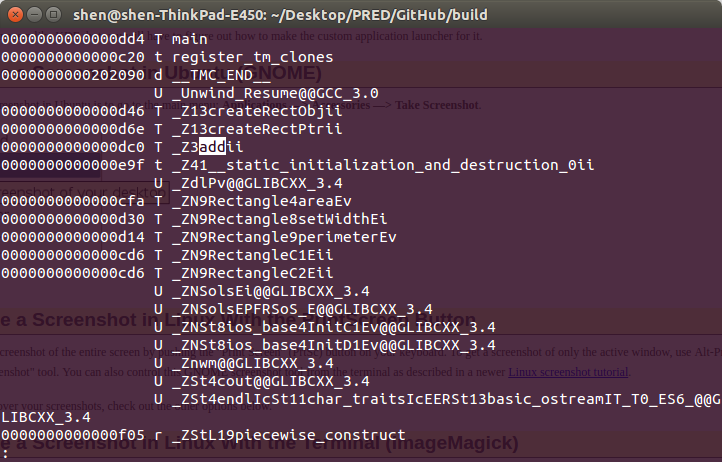
\includegraphics[width=0.8\textwidth]{Images/nmCommand}
     
   \caption{Determinate symbols in shared object}
   \label{fig:nmCommand}
\end{figure*}


\subsection{SWIG}


\section{C++ template}
\begin{lstlisting}
#include <iostream>
#include <sstream>
using namespace std;

//declaration of a class template
template<class T> class Rectangle {
  private:
    T width, height;

  public:
    Rectangle (T, T);
    T area ();
    T perimeter ();
};

//definition of the constructor in a template class
template<class T> Rectangle<T>::Rectangle (T a, T b) {
	  width = a;
	  height = b;
}

template <class T>
T Rectangle<T>::area(){
	return width*height;
}

template <class T>
T Rectangle<T>::perimeter(){
	return (width+height)*2;
}
\end{lstlisting}

\subsection{Node FFI}
    
    
\subsection{SWIG}
%--------------------------------------------------------------------------------